%!TEX root = ../risk_report.tex

\chapter{Discourse-semantics of \emph{risk} in the NYT} \label{chap:discussion}

Accordingly to SFL, the sum total of lexicogrammar, abstracted, realises the discourse-semantics of texts. Accounting for discourse-semantic meaning involves sensitivity to realised lexicogrammatical forms, but also to the ways in which incongruence and grammatical metaphor can create similar meanings through differing grammatical constructions: as noted earlier, \emph{potential harms} may be realised as a participant in a process of risk (\emph{Bush risked losing the election}), or as a modifier of a risk participant (\emph{the cancer risk\slash the risk of cancer}).\endnote{A key issue in CADS is the ability to systematically account for rank-shifted meanings (See McDonald, Forthcoming).}~Given the diversity of roles in which risk words can appear, the delineation of risk by roles within mood and transitivity systems in the previous section was thus a methodological necessity, but one with heavy ramifications for analysis. At the level of discourse-semantics, it becomes necessary to discuss risk word behaviour more fluidly, with reference to both experiential and interpersonal meanings, and with distinctions between risk as participant, process and modifier largely collapsed. This is perhaps especially so in in our case, as risk is an example of a lexical item that may be congruently realised as either participant and process, straddling the semantic space between entity and event.

The first part of this discussion provides a description of risk in the NYT absent longitudinal considerations---something akin to the descriptions provided by \citeA{hamilton_meanings_2007} and \citeA{fillmore_toward_1992}, but from a systemic-functional, rather than frame-semantic purview. The second part is concerned with accounting for shifting discourse-semantics of risk, via the lexicogrammatical findings presented in the previous section. In the final section, longitudinal shifts are discussed in the context of specific events, broader social change, and sociological theory.

%as well as a brief commentary on the usefulness of sociological perspectives in tandem with SFL as a means of understanding the relationship between text, discourse, language and context.

\section{A monochronic description of risk}

Before turning our attention to the behaviour of risk words over time, it is useful to provide a short description of the way risk words are generally used in the NYT.

Foremost, striking is the ability of risk to function within all open word classes (noun, adjective, verb, adverb), as well as the sheer diversity of risk words. 507 unique lexical items containing risk were found\endnote{This naturally depends on your definition of a word\slash token. If we removed hyphenates or tokens containing a slash (\emph{risk\slash reward}), the list would be dramatically reduced in size. Lemmatisation would compress this list even more.}, including many (albeit vary rare) words lacking existing lexicographical description: examples such as \emph{risk-shy}, \emph{risk-addicted}, \emph{risk-elimination}, \emph{species-at-risk} and \emph{risk-happy} demonstrate the overall salience of risk and the nuance with which it is instantiated in news discourse. Further testament to this salience are the nuanced distinctions in riskers' awareness of potential harm in \emph{risking}, \emph{putting at risk, }\emph{taking} and \emph{running} risks.

In many respects, our findings agree with those of other monochronic descriptions of risk language. First, we can see the usefulness of the frame-semantic categorisation of the kinds of participants\slash social actors that occur within the risk frame \cite<i.e.>{fillmore_toward_1992}: we often found it useful to divide corpus interrogation results into categories of \emph{risker}, \emph{potential harm}, \emph{risked thing}, and the like. Promising is the fact that in many cases, we can use the grammatical structure of the clause to automatically return lists of each kind of participant. In cases where the grammar alone cannot tell us the participant role (\emph{I risked my death}, \emph{I risked my life}), manual sorting is not difficult, as there is little ambiguity. If we insert the \emph{losing} participle (\emph{I risk losing my life}, but *\emph{I risk losing my death}), we can quickly determine if a result is a \emph{potential harm} or a \emph{risked thing}. This is especially so when risk is the \emph{process}, rather than a participant or modifier. With this in mind, focussing more exclusively on risk as process in very large parsed datasets may prove elucidating.

Our findings also agree with a key claim made by \citeA{hamilton_meanings_2007}: health and illness risks were surprisingly prominent within our data. As will be discussed below, however, this does not appear to be a purely static phenomenon: our longitudinal analysis points toward health risks as being far more common in contemporary language than in the language of our 1963 dataset.

A second point on which we agree is with their contention that risk words behave differently in different social situations (i.e \emph{registers}) and different genres, and that comparison of genres is worthy of further study (though here we rely on not on our dataset but on a long history of research in support of this contention within SFL):

        \begin{quote} \small \singlespacing
        We find in these discourse environments that the focus of the semantic prosody and the semantic preference changes according to the context in which they occur. While this may be something that some (but not all) sociologists of risk may have intuitively sensed in the past, there are empirical data from corpus linguistics to suggest now that the semantic prosodies can and do change slightly from one context to another \citeyear[p.~177]{hamilton_meanings_2007}.
        \end{quote}
        %
        Their dataset included transcribed spoken conversations. This register is remarkably different to that of NYT articles, and examples of risk in these contexts demonstrate this quite clearly (e.g. \emph{Don't don't risk it eh}; \emph{Cos there isn't a risk of going of there}). The key characteristics of these examples (informal lexis, unrecoverable deictic references, low lexical density, etc.) contrast starkly with our examples.

        Due to the composition of our dataset, we can have little to add to descriptions of risk in casual spoken language, aside from recognising that spoken risk talk is likely to point toward very different, and interesting, results. Though we believe our results may be generalisable to the behaviour of risk in relatively formal written contexts, extended investigation of risk in spoken corpora remains needed.

        A key finding that received little attention in this earlier linguistic research of risk language is the notion of participants' \emph{agency in risk}. Consider the following two sets of examples. The first, from 2012, shows examples of the embedded process as negative outcome.

\begin{enumerate}    [before=\itshape,font=\normalfont] \setlength\itemsep{0em} \small
        \item Some Democrats are saying the White House set itself up for the charges by making a vow that was bound to be difficult to keep and that would \textbf{risk alienating} its business supporters.
        \item Some speculated that this partnership \textbf{risked alienating} other big retailers, like 7-Eleven, by giving Starbucks influence over how Square 's payment system was developed.
        \item And campaigning on behalf of members of Congress could \textbf{risk alienating} swing voters, many of whom seem to prefer bipartisan government and dislike one-party rule.
        %\item But Cravath's pay bump will pressure competitors to increase their year-end bonuses or \textbf{risk alienating} their junior lawyers.
        %\item The changes risked alienating some parents, but ratings in certain important demographics have increased 30 percent, according to Nielsen data.
\end{enumerate}
%
The second contains grammatical subjects modified by \emph{at-risk} (from 2008):

\begin{enumerate}    [before=\itshape,font=\normalfont] \setlength\itemsep{0em} \small
    %\item Senate Democratic leaders are pushing a bill to let many at-risk homeowners do just that.
    \item He secured nearly \$100,000 for a program at the Sephardic Community Center in Brooklyn that seeks to help `at-risk immigrant youth successfully acculturate' into American society
    \item Through the years, he said, more than 1,000 at-risk young people have arrived at his doors.
    \item The document signed off on a \$1.5 million grant to World Vision, a group that hires only Christians, for salaries of staff members running a program that helps `at-risk youth' avoid gangs.
\end{enumerate}
%
Readily apparent when risk is process is that the kinds of people who risk are typically institutions or humans in positions of power and influence. Actors of risk processes are often states, politicians, or political parties. The \emph{potential harm} being risked is often an abstract concern: \emph{alienating} or \emph{offending} \emph{electorates} or \emph{allies}. In these cases, risk is a process engaged in purposively by Actors who stand to gain something equally abstract. In contrast, when risk functions as a modifier of a participant, the participant is far less powerful: women and children are at-risk of sickness; workers are at risk of injury or death. Here, risk is a quality ascribed to the self. Risky behaviour is not often mentioned. For these people, the potential harm is often recoverable from context, but not outlined within the clause. This distribution was largely consistent throughout our dataset, and will be unpacked through sociological analysis in the following chapter. % note that this may change... 

\section{Shifting discourse-semantics of risk in the NYT}

    Some lexicogrammatical and discourse-semantic phenomena have demonstrated consistent shifts over our sampling period. We turn our attention to them now.

    First, though we noted above that risk as a process involves a different set of participants to risk as a modifier, there are still longitudinal changes within this area. When looking at the \emph{risk of loss}, for example, we can see a general trend toward individual losers, rather than institutional losers. In the 1963 data, the things at risk of loss are macro-level and abstract: \emph{athletic funding}, \emph{market share}, \emph{vital technology}, \emph{sympathy in the west}, and the like. Later, risked things are more individual assets---\emph{life} and \emph{injury} being the two most common. We link this conceptually to neoliberalism


    \subsection{Experiential role of risk words}


There is a major functional-semantic difference between risk as a participant and risk as a process. As a process, when the direct object is the valuable object\emph{risk} may be nearly synonomous with \emph{jeopardise} (\emph{I risk my life}). When the direct object is the negative outcome, risk as a process means `may potentially face\slash incur\slash suffer', with a negative connotation.

Risk as a participant typically stands in for the potential harm, rather than the actual process that may result in a favourable outcome.

To better understand the difference, we can concordance nominal `benefit', which shows that risk as a parti

as in Filmore and Atkins' frame, the end result of a risk process is either the goal/benefit or the harm/negative outcome.

When risk is a participant, however, it generally stands in for only the harm/negative outcome: the risk was outweighed by the benefit

the risk/reward ratio is another example: again, in this case, risk \emph{is} the potential harm.

The riskier something is, the more likely the negative outcome. In many cases, the goal may be exponentially greater, but this is not the 

There are very few examples in the data where a risk itself has benefits. Instead, risk and benefit are converse, joined through conjunction: risk or benefit, risk and benefit, risk but benefit, but rarely 

\begin{quotation}
An array of new techniques, each with its own risks and potential benefits, makes for bewildering options for women.
\end{quotation}

When risk is a process, benefit and reward refer to specific schemes:

\begin{quotation}
The Kaziyevs were told they had 10 months to become citizens or risk losing Medicaid benefits.
\end{quotation}

\begin{quotation}
Once the marriage ban in New York State is lifted, domestic-partner couples , both gay and straight , will risk losing access to health care and other benefits if their employers treat marriage as the only ticket for entitlement to these benefits, which are increasingly expensive.
\end{quotation}

Because of this difference, a shift toward nominal forms is in itself a shift toward a semantic conceptualisation of risk as more interchangable with harm itself.

The recent discussion about risk's becoming more or less interchangeable with threat is not fully supported by the data.

A risk of anything is a risk of harm. 

Risk as a process can contain within its adjuncts (or, less likely, within a complement) the goal, or positive outcome. Risk as a participant cannot. When it co-occurs with the goal, the relationship between them is through coordinated conjunction.

As our corpus was built from paragraphs containing risk words, we lacked resources to sufficiently test whether risk behaves more or less like related words such as \emph{threat} or \emph{harm}. Such an investigation, using a substantially larger corpus, is planned.
    
    \subsection{Domains of risk disourse}

           \begin{figure}[htb!]
            \centering
            \addvbuffer[12pt 0pt]{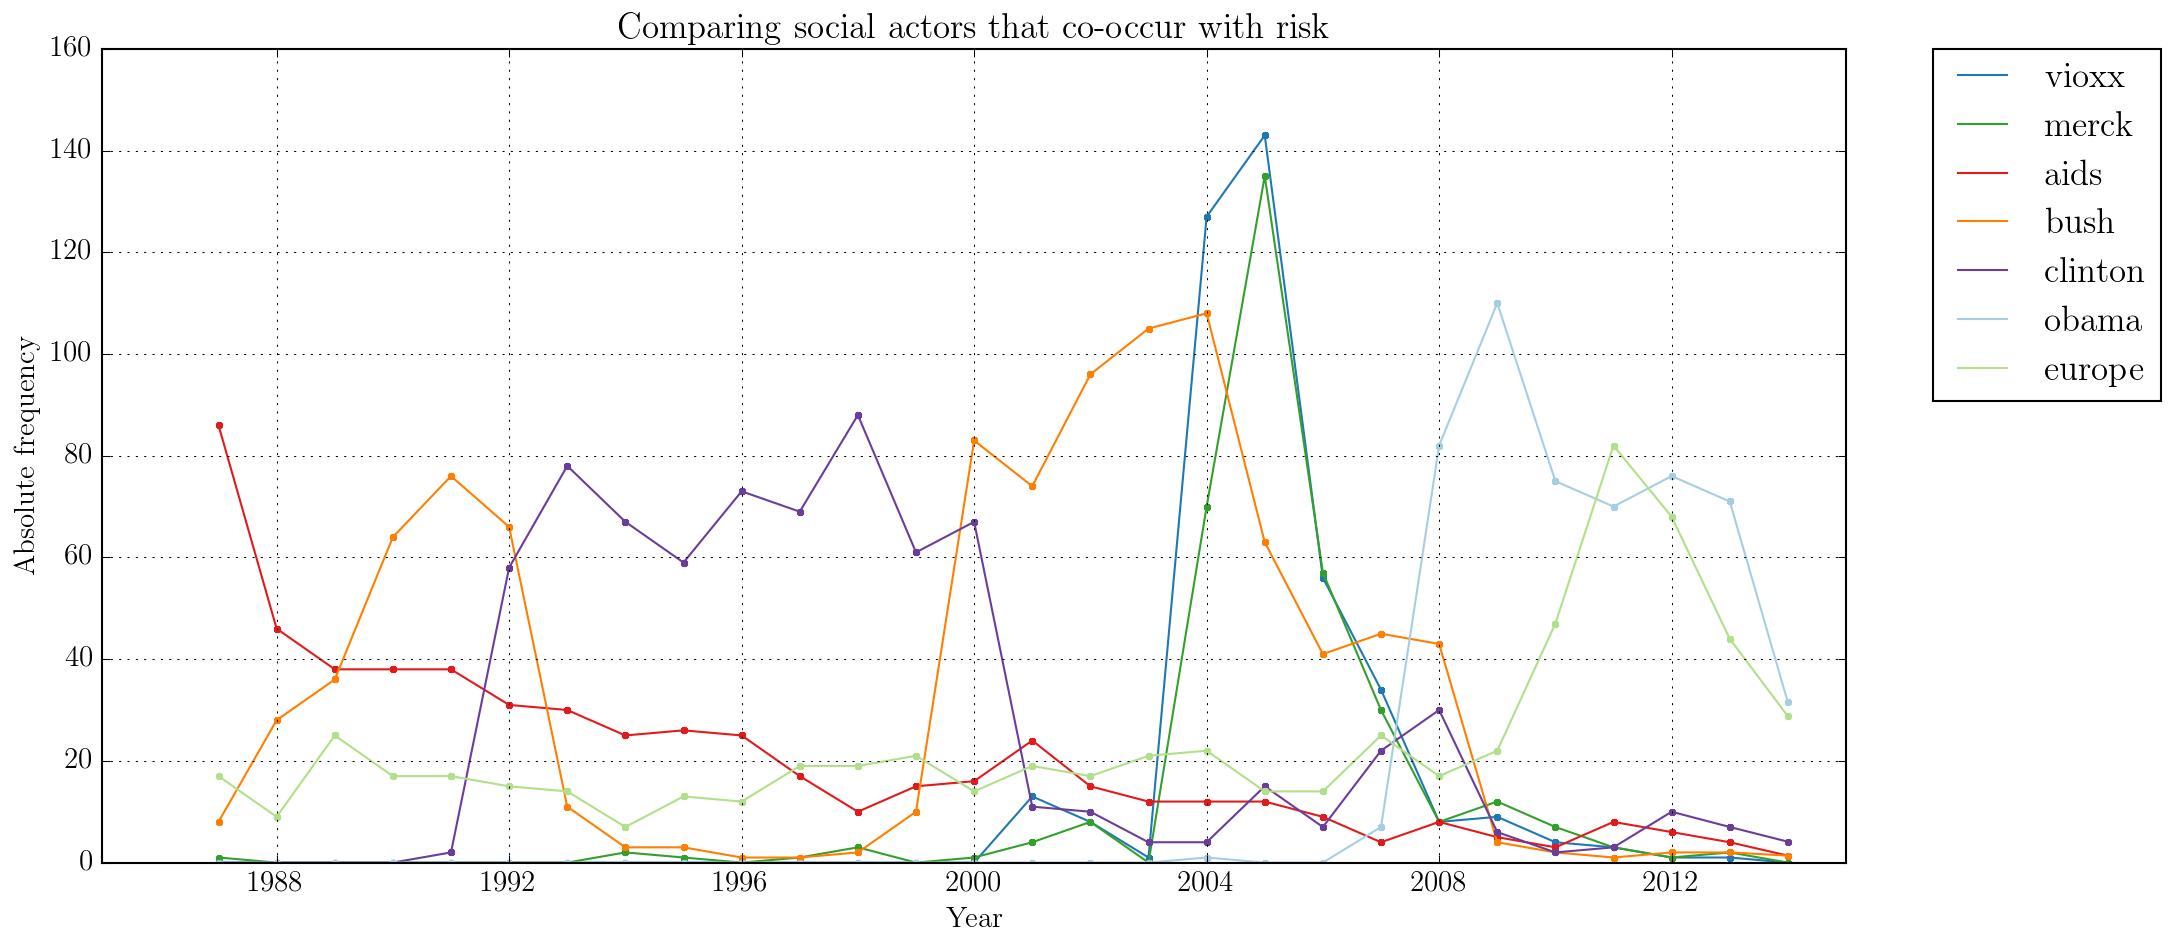
\includegraphics[width=0.75\textwidth]{../images/comparing_social_actors_that_co-occur_with_risk}}
            \caption{Comparing social actors that co-occur with risk}
            \label{fig:comparison}
            \end{figure}

        In terms of the topics in which risk words are deployed, we saw that health risks are very prominent in the more contemporary data samples. Our comparison of \emph{Risk of terror* attack} and \emph{risk of heart attack} demonstrates this preference clearly. This change is indeed a longitudinal one: in 1963 editions, a number of constructions evidence that risk was commonly instantiated with regard to diplomacy, war, international relations, and the like. In their most prominent years, AIDS, Vioxx and Merck comprise over 1.6 per cent of all proper nouns that co-occur with a risk word. This is higher than Clinton, Bush or Obama at their peaks, as well as Soviet Union in 1963\slash 1987 or Europe during the Eurozone crisis in 2011 (See Figure \ref{fig:comparison}). Moreover, in the years following the AIDS crisis, health risk have increasingly related not to infectious diseases (which require institutional responses), but to kinds of illnesses where the responsibility for prevention falls upon everyday citizens through lifestyle choices, rather than politicians, hospitals, or the FDA. Even in the case of Vioxx, where the risk was created by the premature FDA approval, risk language surrounding Vioxx remained geared toward the risks faced by everyday people. Though Merck and the FDA may be blamed, risk remains a more appropriate frame for discussing the potential for heart attack than it does for discussing the potential harm caused by improper clinical trials or financial interests causing the FDA to approve the medication prematurely\endnote{Future research will centre on unpacking the kinds of agents involved in healthcare risks of HIV, AIDS, Vioxx, etc.)}. In hundreds of co-occurrences of risk words, Vioxx and Merck, we uncovered a mere handful where the potential harm was to the manufacturer. Though we found one solid example in the 2006 subcorpus (\emph{`The verdict highlights the \textbf{risks} that Merck faces as the number of lawsuits over Vioxx continues to grow.'}), this same article containined four other risk words, each of which positions the consumer as being subject to potential negative outcomes:

        \begin{enumerate}  [before=\itshape,font=\normalfont] \setlength\itemsep{0em} \small
            \item Mr. Escobedo said that Vioxx was especially dangerous to Mr. Garza because of his other \textbf{risk} factors and that he should never have been prescribed the drug.
            \item `Mr. Garza was the last person in the world that should have been taking Vioxx,' said Mr. Escobedo, who told the jury that Merck had known since 2000 that the drug posed heart \textbf{risks} but continued selling it for four years.
            \item About 20 million Americans took Vioxx from 1999 to 2004, when Merck withdrew the drug after a clinical trial showed that it increased the \textbf{risk} of heart attacks and strokes compared with a placebo. Earlier clinical trials had also shown that Vioxx appeared to be much riskier to the heart than naproxen, an older painkiller.
            \item But recently the tide has seemed to turn abruptly against the company, as its lawyers struggle to explain a raft of documents that show its scientists were concerned about Vioxx's heart \textbf{risks} several years before Merck stopped selling the drug in 2004. 
        \end{enumerate}
     
        As \citeA{widdowson_limitations_2000} suggests, corpus linguistics often reveals things that are contrary to intuition, and this is certainly the case here. Our expectation of new risk meanings related to terrorism after 9\slash 11 was for the most part not met. Rather than a limitation, this can be treated as an insight in itself: the events and topics that come to mind when we think of risk may not necessarily correspond to the reality of risk language generally. Such is the benefit of corpus linguistic investigation of risk, when compared with previous methodologies employed within the humanities and social sciences to better understand risk.

    \subsection{Implicitness and arguability}

	   The most salient theme from the longitudinal mapping of risk is that of implicitness: increasingly common are grammatical constructions where potential harms and risked things are recoverable only from context. Below are three further examples of the \emph{at-risk} construction:

        \begin{enumerate}    [before=\itshape,font=\normalfont] \setlength\itemsep{0em} \small
            \item In 1999, we sold the company, and the next year, we moved to the United States with our two children---a third was born in 2003---so I could pursue my idea of helping low-income, \textbf{at-risk youth}.
            \item Some of the proceeds from tickets sales for the event {[}...{]} will go to support local arts programs in Washington Heights and the Broadway League's Family First Nights, which the League describes as `a nationwide program specifically designed to encourage \textbf{at-risk families} to attend theater on a regular basis.'
            \item Mr. Tepfer noted that Mr. Douglas, who was in the neighborhood when the body was found and was interviewed by the police at the time, `preyed on \textbf{at-risk women}, on prostitutes, and he engaged in sex and strangled them to death.'
        \end{enumerate}
        %  
        In these cases, what the participant is at-risk \emph{of} is not a specific negative outcome, but an interrelated set of negative outcomes that are more likely to happen to less powerful people in society. Evoked within this cluster is \emph{poverty}, \emph{drug use}, \emph{disease}, \emph{homelessness}, \emph{abuse}, \emph{fatherlessness}, \emph{dropout}, \emph{gang activity}, and the like. In many cases, \emph{at-risk} takes on a euphemistic quality, most obviously as a substitute for \emph{lower-class}, \emph{non-white} or \emph{poor}. Also interesting here is the muddying of the semantic frame: it is both difficult to determine the exact potential harm, and to classify the participant as a \emph{risker}, which seems to imply some agency or comprehension of the risk. More accurately, these participants are \emph{put at risk}---a risk process that itself is on an upward trajectory within our dataset.\endnote{Indeed, this is aligned with recent changes to the frame semantic conceptualisation of risk. At the time of writing the FrameNet entry for \emph{run risk} included the following caveat: `\emph{NOTE: This Frame is currently in the process of being changed so that some instances of at risk.n will be moved to the Being\textunderscore at\textunderscore risk frame, and some will be moved to the Risky\textunderscore situation frame. In the Being\textunderscore at\textunderscore risk frame, risk is almost always supported with at, and its external argument is the Asset}' \cite<see>{baker_berkeley_1998}.}~ 

        % https://framenet.icsi.berkeley.edu/

        This aligns with the decreasing arguability of risk. Risk in predicator or subject position is increasingly rare, as risk becomes less the nub of propositional meanings. Thus, less and less often is risk a fundamental component in meaning as exchange: in its role within complements and adjuncts, it now more typically plays a supporting role in the provision of information. A ramification of this is that risk becomes an inherent quality of participants in the field of discourse, rather than a process in which participants knowingly or by their own choice choose to engage. This shift is exemplified by the outbound trajectory of \emph{calculated risk}, and its displacement by an uncalculated \emph{potential risk}. Below are examples of \emph{calculated risk} in 1963, contrasted with \emph{potential risk} in 2008.

        \begin{enumerate}   [before=\itshape,font=\normalfont] \setlength\itemsep{0em} \small
            \item It is, of course, a \textbf{calculated risk} that Mr. Kaye is taking.
            \item Kennedy has taken a \textbf{calculated risk} here.
            \item A spokesman for the group acknowledged that granting a 10 per cent discount before a study in depth had been made was a calculated risk.
        \end{enumerate}

        \begin{enumerate}   [before=\itshape,font=\normalfont] \setlength\itemsep{0em} \small
            \item One was to make health care providers and caregivers of infected children aware of the \textbf{potential risk} of pre-chewing.
            \item At issue were the \textbf{potential risks} of having government-run funds in China and other foreign countries make big investments in American businesses.
            \item Rat pups exposed to BPA, through injection or food, showed changes in mammary and prostate tissue, suggesting a \textbf{potential cancer risk}.
        \end{enumerate}

        In the former, the existence of the risk itself has been acknowledged, and the potential harm\slash reward have been weighed. In the latter, though the situation can be identified as having potentially negative outcomes, these are formless and immeasurable. This aligns with the idea that risk (sociological reference) has come to be simply \emph{threat}.

        % It is an unspecified potentiality while calculated risk implied a degree of control.

        \subsection{Low-risk, moderate-risk, high-risk}

        \begin{enumerate} [before=\itshape,font=\normalfont] \setlength\itemsep{0em} \small
        \item Hemophiliacs, at \textbf{high risk} of AIDS, have been hard hit by the disease.
        \item Another 25 percent are \textbf{at moderate risk}.
        \item But why on this isolated campus, where no AIDS cases have been reported among students at \textbf{low risk} of catching the disease, are students so concerned?
        \end{enumerate}
            %
            During the first years of the U.S. spread of HIV, people could be classed according to low, moderate and high-risk groups. Here we have basic quantification of levels of risk. This stands in contrast to the \emph{at-risk} construction discussed above. Of these modifiers, only \emph{low-risk} emerges as an increasingly frequent form. This is also interesting, as it points to a broadening of the semantic scope of risk to include situations where risk remains present: \emph{low-resolution image} does not point toward the increased prominence of low resolution images, but more to the prominence of resolution as thing that meanings are made about. In the same way, the inward trajectory of \emph{low-risk things} does not point toward a culture of less risk, but toward a culture where even things that do not have risk are characterised by their nature to it. We could not locate existing literature supporting a claim that the salience of a concept may be evidenced not only through \emph{extreme case formulations} \emph{the riskiest, high-risk, very risky}, but through minimisation. Nonetheless, our analysis points to the idea that the increased salience of risk as a concept is in part demonstrated through its instantiation in situations where its significance is claimed to be negligible or banal.

            \subsection{Risk as modifier}

            \begin{enumerate}  [before=\itshape,font=\normalfont] \setlength\itemsep{0em} \small
                \item At JPMorgan Chase, the \textbf{risk models} hid---and were used to hide---risks from the traders and top executives.
                \item After a rogue trader cost MF Global \$141 million, Promontory came in to bolster certain areas of the firm's \textbf{risk controls}.
                \item He was a total \textbf{risk junkie}.
                \item The programs are all based on the concept of risk management, rather than the unattainable goal of total \textbf{risk elimination}.
            \end{enumerate}

            Risk occurs within many different modifier positions (see Table \ref{tab:modriskwords}). Of these, pre-head nominal types are rising, and adjectival pre-head types are falling. From these shifts, we can surmise some sociological insight related to arguability (as conceptualised by SFL). In the increasing frequency of pre-head nominal modifiers (\emph{risk management, risk arbitage, risk factor, risk insurance}---more examples above), we can see increased social significance of risk as a concept through the evolution of specific jobs whose central concern is risk (see Section \ref{sect:riskmod} for discussion of the emergence of \emph{risk factor} in particular). Pre-head nominal modification reflects the codification of a concept: such constructions must be culturally recognised constellations of meaning. In comparison, adjectives attach to head nouns relatively freely in English. Cultural recognition of the adjective-noun combination (\emph{a risky move}, \emph{the riskiest option}) is not a prerequisite for meaning to be understood.

            \subsection{Arguability} \label{sect:arg}

            Longitudinal change in the arguability of risk words is consistent. In earlier editions, risk words more commonly occupy more arguable roles, according to systemic functional grammar. In later editions, risk more commonly occurs in heavily dependent positions. Less often does a risk word form the central component being discussed; more often, it exists as a modifier of one of these components, or as a part of a supporting, subordinate clause.

            Increasing nominalisation and `participantification' of risk (See Figures \ref{fig:wordclasses} \& \ref{fig:funcrole}) are also indicative of decreased arguability. The key affordance of nominalisation is that it reduces the need to make meanings through constellations of Participants and Processes: instead, 



            Given that Processes in the Transitivity system pattern with the Finite\slash Predicator in the Mood system, nominalisation facilitates clauses with larger amounts of less arguable information.

            The discursive function(s) of nominalisation are well-acknowledged both within SFL and outside of it.

            `The interpersonal price of decreasing negotiability' (Halliday \& Martin, 1993, p.~41)

            Nominalizing `allows the writer to give the required flavor of objectivity to his or her statements and claims' (Holes, 1995: p. 260). 
            Nominalization disengages the speaker/writer from commitment to the truth of his/her statements by allowing him/her to make `unattributable claims' (Quirk et al, 1985: p. 1289);
            Nominalization has the capacity to blur/mystify agency, thus `masking real intentions' (Hatim, 1997: p. 114);

            %Hatim, B. (1997). Communication across cultures. Translation theory and contrastive text linguistics. Exeter: University of Exeter Press.
            %Hatim, B.  \& I. Mason (1997). The translator as communicator. London and New York: Routledge.
            %Holes, C. (1995). Modern Arabic: Structures, functions and varieties. London/New York: Longman.
            %Quirk, R., S. Greenbaum, G. Leech \& J. Svartvik (1985). A comprehensive grammar of the English language. London: Longman Group Ltd. 
            %Stubbs, M. (1998). Language and the mediation of experience: Linguistic representation and cognitive orientation. In F. Coulmas (Ed.), The handbook of sociolinguistics (pp. 358-373). Oxford: Blackwell. 

            We are limited in our ability to interpret this result. Little has been written about the relationship between dependency grammars and SFL. As dependencies are inherently functional-semantic, rather than generative-grammatical, dependency is perhaps the most useful \endnote{Current systems for automatic systemic functional annotation tend to rely on dependencies generated with Stanford CoreNLP} mainstream grammar for learning about the semantic behaviour of a given word. That said, though functional categories provided by Stanford CoreNLP's dependency parser overlap in many respects with categories in the Mood system of SFL, there are still mismatches, or shortcomings. Most critically, dependency grammar conflates interpersonal, experiential and textual systems, while SFL demands three separate parses. As discussed earlier, the systemic-functional conceptualisation of subjecthood is threefold, whereas CoreNLP simply nominates the interpersonal subject.

            Due to the availability of nuanced querying languages for phrase structure grammar annotation, our investigation leaned toward grammatical structure annotation over dependency grammar. This is despite a problematic relationship between functional and phrase structure grammars. Given that interesting preliminary findings were unearthed by querying dependency information, we conclude that further exploitation of dependency annotation for the purpose of risk language analysis appears to be a promising area for further analysis.

    \section{People and risk}

    A particular strength of our approach is that it is possible to understand nuanced distinctions in the ways in which social actors are related to risk. Looking specifically at words pertaining to normal, everyday people (\emph{person\slash people}, \emph{man\slash men}, \emph{woman\slash women}, \emph{childs\slash children}, etc.), we can see that

    Using linear regression to calculate which words in which contexts are becoming increasingly frequent or infrequent throughout our sampling period, we can see that everyday people behave 

    As seen in the health corpus, everyday people are associated more and more with risk discourse: this class of nouns is becoming more frequent, overtaking words related to institutions. When looking specifically at who is the actor in risk processes, however, a different picture emerges: banks, agencies and companies are becoming more frequent, while everyday people 

    This finding paints a rich picture of the changing discourse-semantics of risk, whereby risks are created through the actions of powerful people and institutions, but, increasingly, suffered and endured by people. This aligns with neoliberal sociological conceptualisations of the distinction between late and reflexive modernities.

	\section{Sociological perspectives}
            
	The task that remains is to connect observed shifts to their temporal context. In terms of the annual subcorpora, this was by no means a clear-cut task. Spikes in specific terms may correspond with particular events, but general shifts in meaning change place concurrently, and thousands of datapoints overlap and intertwine with the points of interest.

	When focussing on the subcorpora of health risks, linguistic reactions to real-world events were easier to locate. We concluded that further investigation of risk would do well to focus on risk as instantiated within texts sharing a semantic field. 

    Our investigation of topic subcorpora was limited by scope. That said, the open-source tools we have developed for interrogating corpora for discourse analysis could easily be put to use in an investigation of a topic subcorpus.

	%~\ \todo[inline,color=green!40]{\noindent Mapping events to risk instantiation in the topic subcorpora here}
	
	We found little evidence that health crises resulted in increased frequency of risk in articles centred on economics or politics. This seems to suggest that while real-world events influence the instantiation of the risk semantic, this instantiation remains more or less limited to the field(s) of discourse to which the real-world event is most related.

	A final point of interest is that adjectival risk words in some respects behaved contrary to our expectations. Simple adjectival risks as modifiers of participants (\emph{the risky manoeuvre}, \emph{riskier choices}) appear to be decreasing in frequency. Furthermore, though there is a very large variety of adjectival risks, and though there is a general trend toward a greater number of risk adjectives, this increase is a slight and gradual one.

	Perhaps in this finding there is some evidence for the Risk Society thesis, in that the ways in which risk can characterise a situation were more or fully articulated during high modernity. Though these characterisations continued to be applied today, saturation point may have been reached.

\subsection*{From positive risk taking to exposure to risk}

It is difficult to automatically identify positive and negative portrayals of risk through querying or concordancing, as much of this sentiment may be carried in the clauses preceding or following a risk word. That said, we can nonetheless note a number of findings which point toward a reduced agency in participation within risk scenarios.

exposure to risk is implied in the \emph{at-risk} construction: very rarely are things at-risk due to a conscious choice by everyday people:

Especially notable is that many constructions that are rising in relative frequency exist without any explicit, or even imaginable, potential goal\slash positive outcome in the risk scenario. Those at risk of disease are not taking a gamble that has any potential pay-off.

Money may be risked, but cannot be put at risk by investors.


\subsection*{Expected risk taking but lacking control}

This hypothesis is partially confirmed by our data. The increasing use of risk language within everyday life world concerns suggests ...

On the other hand, the shift from infectious to non-infectious diseases within health risks is accompanied by 


through journalism, people are educated about which factors are within and outside of their control.

Given that factors beyond the control of individiduals play a significant role in their likelihood of developing heart disease or cancer, 





A complicated picture emerges, where individuals are indeed charged with the task of managing their health risks, and yet, the kinds of negative outcomes they are attempting to prevent are in large part caused by factors beyond their control.



The key semantic distinction between different risk processes is the extent to which the risker is aware of the potential for a negative outcome, or able to choose to participate in the process of risking or not.





\subsection*{The increasing salience of at-risk status in risk reporting}

A limitation imposed 

Though a key way in which increased salience may manifested itself in language is through increasing use of \emph{at-risk} as the head of the Subject or the Finite\slash Predicator of a clause, this is rarely grammatical in English. Accordingly, our test for increased salience is centred on increasing usage generally.

\subsection*{Individualisation winners and losers---risk-takers versus at-risk groups}






    %\emph{What can be concluded from the finding that real world events do not appear to have long-lasting effects on the behaviour of risk words?}

    %Ultimately, perhaps we should not be surprised by this finding. Language is a system that must be resilient against such influences: if single events caused meaningful changes in the lexicogrammatical behaviour of a single word, communication between those aware of and unaware of events would be made more difficult. Accordingly, our suggestion would be that temporary change in the behaviour of a word (as can be seen in spikes in the number of risk words surrounding certain events) are interesting in and of themselves. Moreover, these changes can potentially be measured in pseudo-real-time by mining RSS feeds, using the Twitter API, and so on. Lexicographers could take note of which kinds of events bring about instantiation of a certain word or concept, and create definitions accordingly. Discourse analysts and sociologists could hypothesise the co-occurrence of certain kinds of language with certain kinds of events, and use real-time data to confirm or refute these hypotheses. Cooperative efforts between functional linguistics and sociology, however, are dependent upon a reconciliation of divergent conceptualisations of the relationship between text and context. This issue is elaborated below.



% Another major finding, unerthed during our investigation of the health subcorpus, was a shift in the potential benefit that may accompany a risk.

% The risk frame identifies the `goal' as the favourable outcome of a risk process, opposed to the `harm'.

% Based on our knowledge of a culture, many parts of the semantic frame can be implicitly understood: in \emph{They risked their money at the casino}, we understand the potential harm losing money) and potential goal (winning money). 

% Concordancing nominal `benefit(s)' revealed, however, unexpectedly revealed that benefit is not juxtaposed against harm, but against the risk process itself:
